\subsection{Baseline predictions}

We began by establishing a baseline model for bass guitar tablature generation.
Initially, we utilized a pre-trained checkpoint from the DadaGP paper \cite{sarmento_dadagp_2021} without additional training.

To generate bass-specific outputs, we experimented with various prompts.
First, we provided a single bass guitar note as the initial token, however the model quickly incorporated tokens from other instruments.
This is an issue documented in the GuitarCTRL paper\cite{sarmento_gtr-ctrl_2023} where they used a metric called the UIP score (Unpromped Instrument Presence) to evaluate the model's ability to generate a specific combinations of instruments.
To constrain the output to bass tokens, we modified the logits of non-bass instruments by setting them to $-\infty$.

% FIGURE REPETITIVE GENERATION
\begin{figure}[!ht]
    \centering
    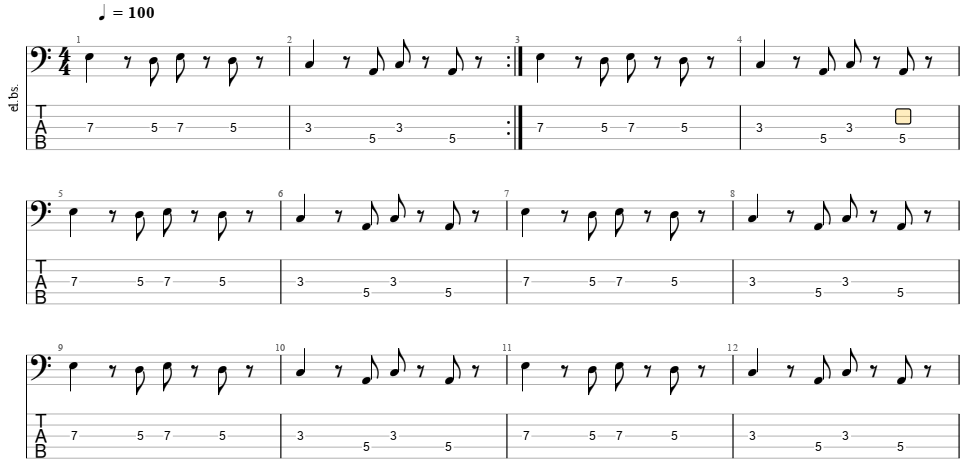
\includegraphics[width=.75\linewidth]{../images-figures/generated_bass_baseline.png}
    \caption{Example of a bass generation from the baseline model}
    \label{fig:repetitive_generation}
\end{figure}

An example of a bass tablature generated this way is shown in Figure~\ref{fig:repetitive_generation}.
While this forced the model to generate only bass tokens, the output quality was poor, featuring repetitive phrases, harmonically incorrect notes, or complete aberrations.
This was expected, as the model was not trained explicitly for bass only generation. 
Unfortunately, we cannot provide a quantitative evaluation of the generated tablatures, as we have not yet defined an evaluation metric.

\newpage

\subsection{BiLSTM - Transformer model}

This section present the results we get using a model adapted from the work of Makris et al. \cite{makris_conditional_2022}.
Our data was adapted to fit the model's input requirements and the model was also slightly modified to fit our task.

% FIGURE MAKRIS ET AL. MODEL
\begin{figure}[!ht]
    \centering
    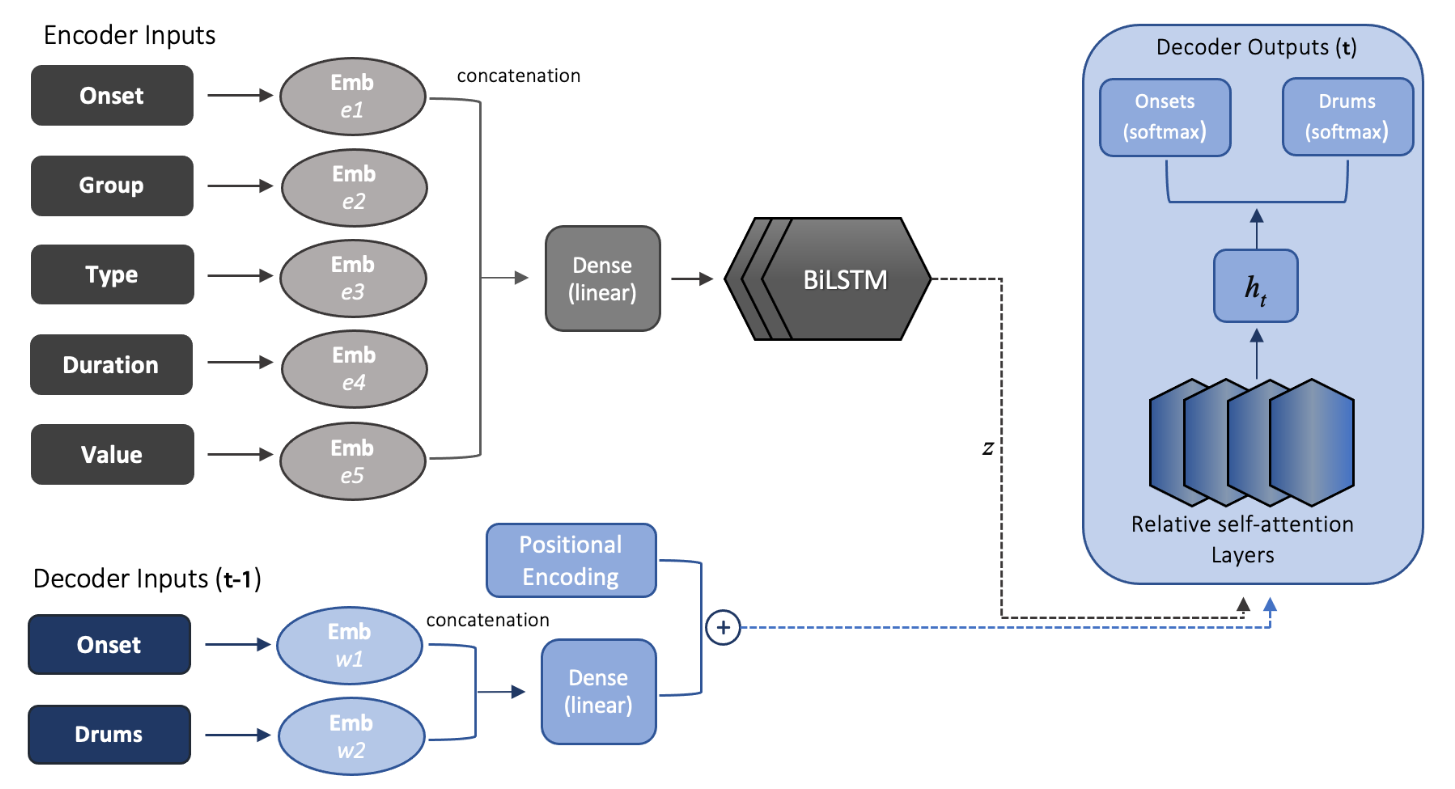
\includegraphics[width=.75\linewidth]{../images-figures/makris_model.png}
    \caption{Makris et al. model architecture, taken from their paper \cite{makris_conditional_2022}}
    \label{fig:makris_model}
\end{figure}

The figure~\ref{fig:makris_model} shows the architecture of the model proposed by Makris et al.
We have presented the compound representation in the state of the art.
This representation concatenates all the parameters necessary to describe a note in a single vector (onset, duration, pitch etc.).

% FIGURE MAKRIS ET AL. MODEL ADAPTED TO OUR TASK
\begin{figure}[!ht]
    \centering
    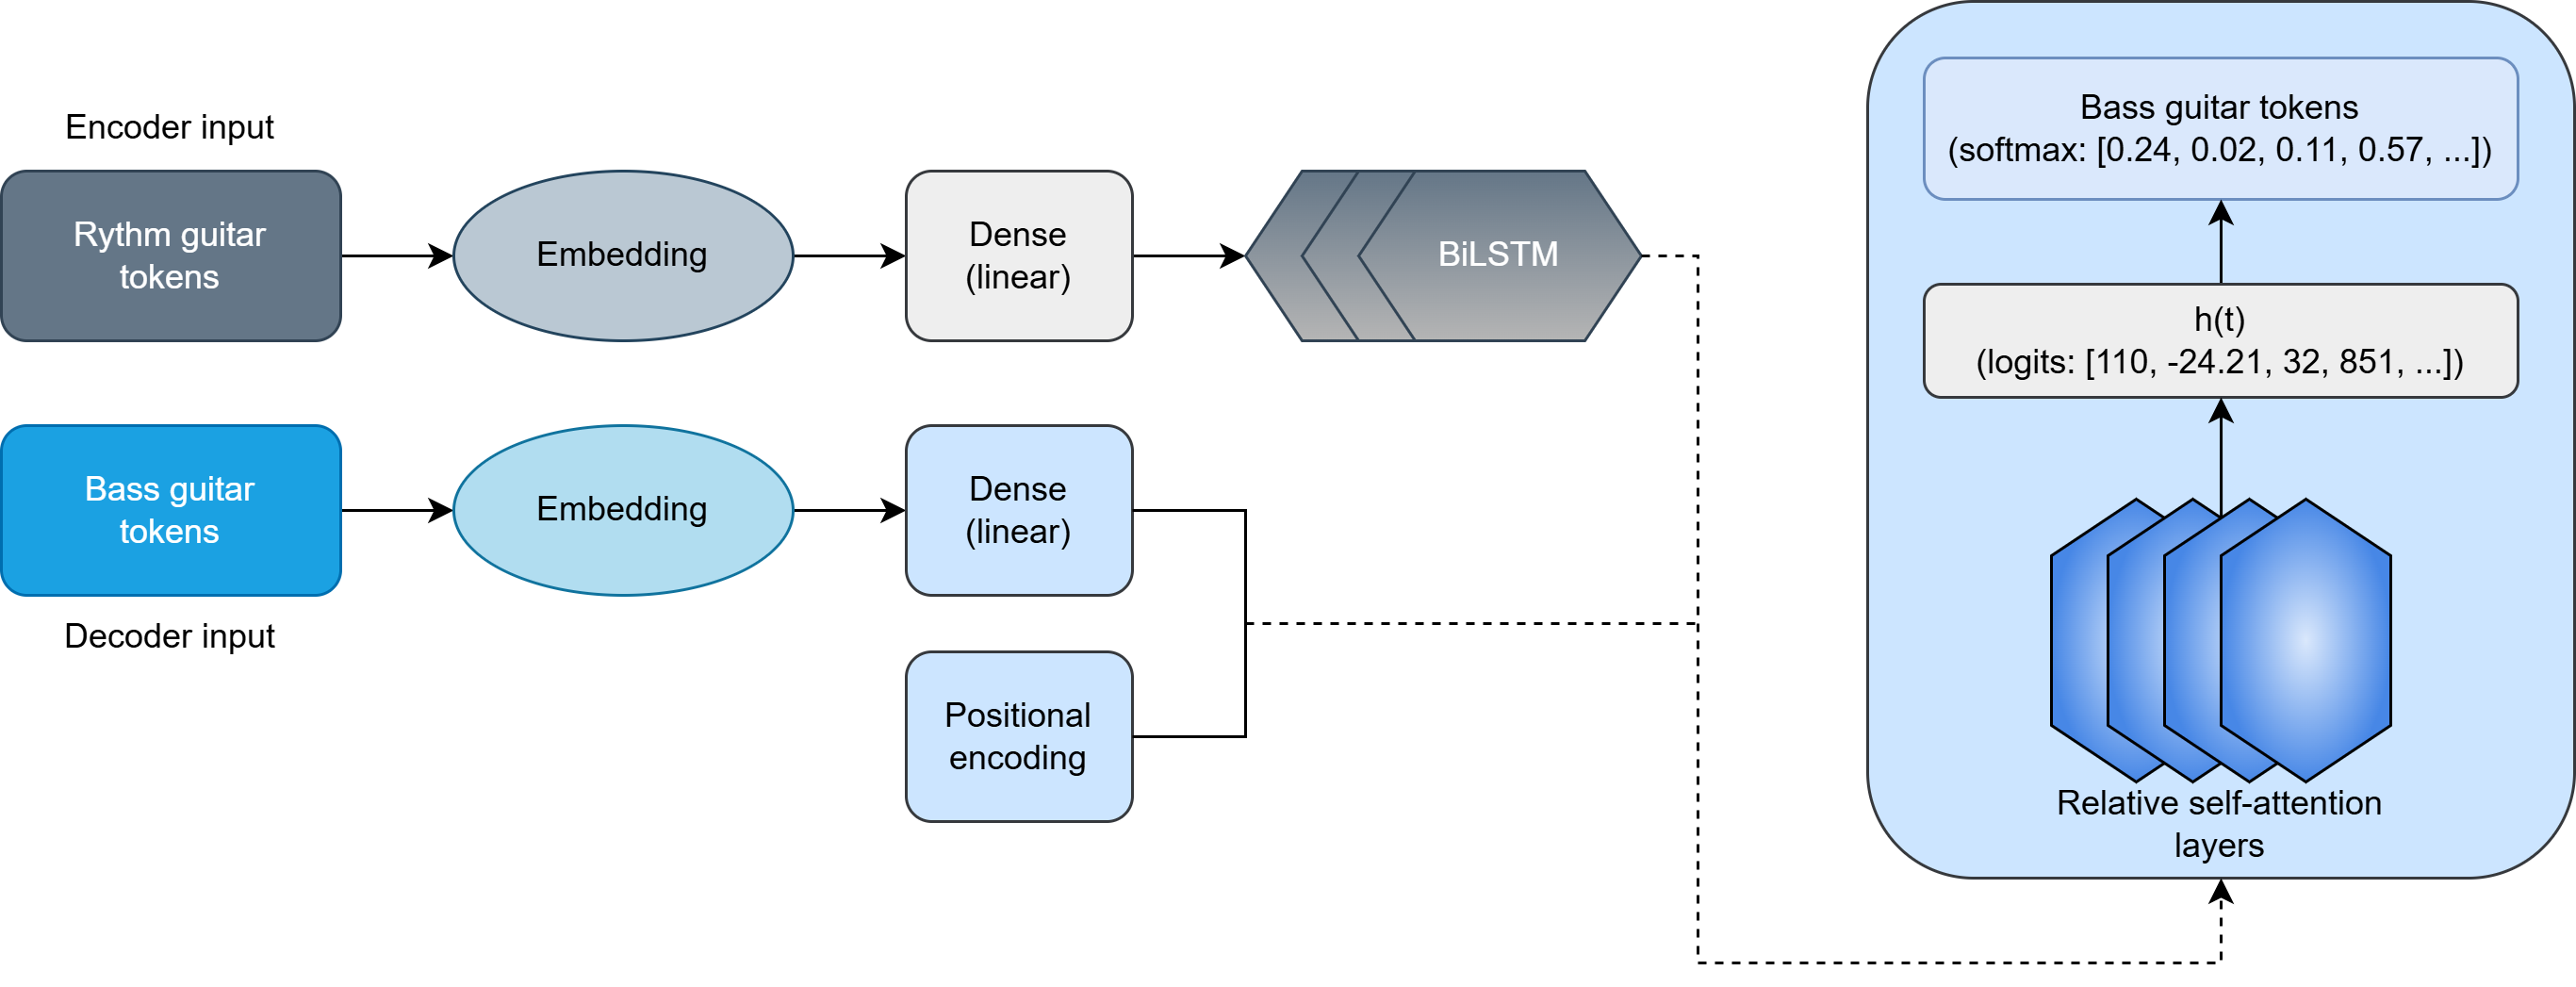
\includegraphics[width=.9\linewidth]{../images-figures/model_adapted.png}
    \caption{Makris et al. model adapted to our task}
    \label{fig:makris_model_adapted}
\end{figure}

Figure \ref{fig:makris_model_adapted} shows the model adapted to our task.
In our case, we have chosen to use DadaGP tokenization which is a different representation.
On the encoder side, the five embeddings concatenated in Makris et al. are replaced by a single embedding in our case.
On the decoder side, the compound word is only made of two inputs because drums notes need much less parameters than other instruments.
They are fully described by their onset and a value indicating the drum type.
This compound representation is also replaced by a single embedding in our case.

The embeddings are then passed through a dense layer. The encoder input (rhythmic guitar) is passed through a BiLSTM layer.
Positional encodings are added to the decoder input and the output of the BiLSTM layer.
All these elements are then passed through a transformer layer with self-attention mechanism
that outputs an array of vocabulary size with the logits of the next token.
These logits are then passed through a softmax layer to get the probabilities of the next token.
All these layers lead to a model of 20 881 514 parameters.


To evaluate our model's performance, we use a loss function based on categorical cross-entropy and an accuracy metric designed for sequence modeling.
The loss function measures how well the predicted probability distribution aligns with the true tokens and is defined as:  

\[
\mathcal{L} = - \sum_{t=1}^{T} \sum_{k=1}^{K} y_{t,k} \log \hat{y}_{t,k}
\]

where \( T \) is the sequence length, \( K \) is the vocabulary size, \( y_{t,k} \) is a one-hot encoded ground-truth token at time step \( t \), and \( \hat{y}_{t,k} \) is the predicted probability for token \( k \).  

Our accuracy metric computes the proportion of correctly predicted tokens in a sequence.
Both functions incorporate a masking mechanism to handle padding tokens and remove their contribution to the calculations.


\subsection{Training}

Training was done on GPU with 200 epochs, an early-stopping criterion of 5 epochs without improvement on the validation loss,
Adam optimizer with the following hyperparameters: $\alpha=5e^{-4}$, $\beta_1=0.9$, $\beta_2=0.98$, $epsilon=1e^{-9}$, and a batch size of 32.

The training stopped at epoch 37 because the validation loss did not decrease anymore for 5 epochs.
We reached 0.97 accuracy on the validation set with 0.14 loss.

% FIGURE EVOLUTION OF ACCURACY AND LOSS DURING TRAINING
\begin{figure}[!ht]
    \centering
    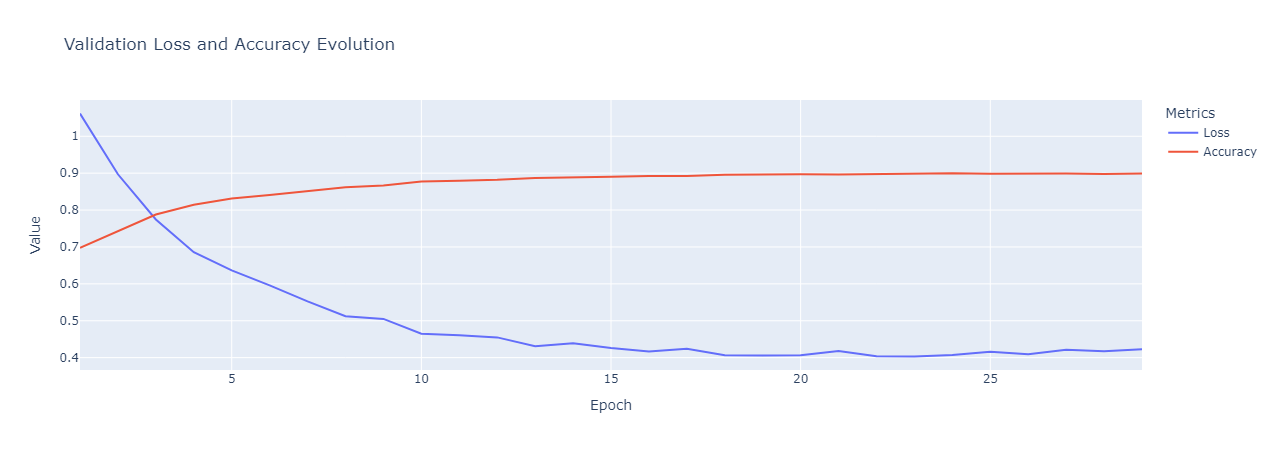
\includegraphics[width=.8\linewidth]{../images-figures/validation_acc_loss.png}
    \caption{Evolution of accuracy and loss during the training}
    \label{fig:validation_acc_loss}
\end{figure}

Figure \ref{fig:validation_acc_loss} shows the evolution of accuracy and loss during training.
The accuracy increases rapidly during the first epochs, then stabilizes around 0.90.